\chapter[Methodology]{Methodology} \label{c:method} 

This chapter outlines the methodology developed for the inverse design of DJ-phase 2D perovskites. Section \ref{section:section3-1} provides an overview of the overall design framework, which integrates chemical space establishment, property prediction, and synthesis feasibility. Section \ref{section:section3-2} introduces the core component of the workflow: an invertible and interpretable molecular fingerprint tailored for organic spacer design. The subsequent sections detail the key pipelines of the framework, including high-throughput calculations (Section \ref{section:section3-3}), machine learning model development and evaluation (Section \ref{section:section3-4}), and the two-step synthesis feasibility screening process (Section \ref{section:section3-5}).


\section{Overview of the inverse design workflow}\label{section:section3-1}

\begin{figure}[ht]
    \centering
    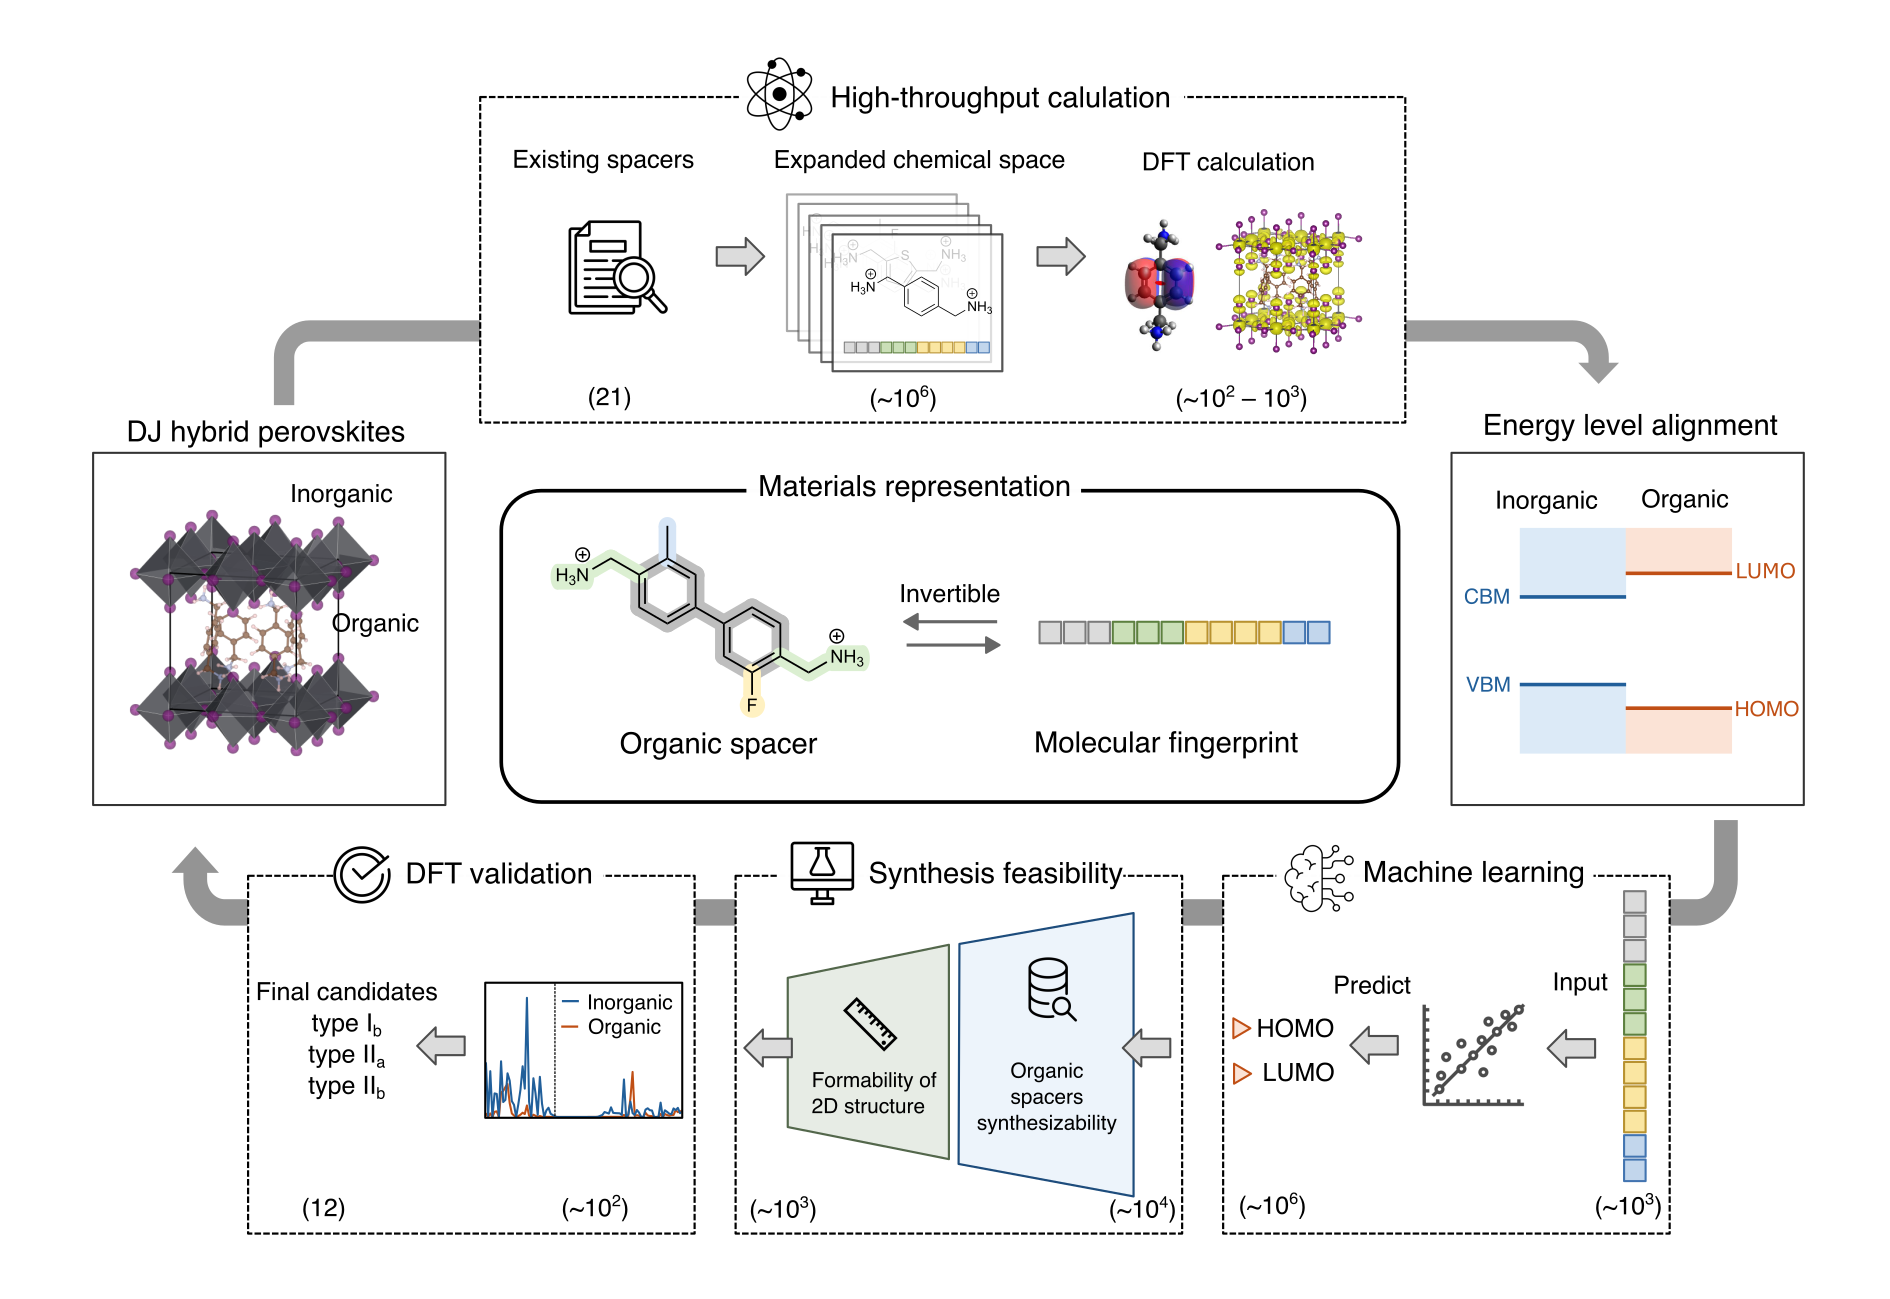
\includegraphics[width=\textwidth]{figures/methodology/figure3-1.png}
    \caption{AI-assisted inverse design workflow for discovering DJ perovskites with targeted energetics and synthesis feasibility. }
    \label{fig:figure3.1}
\end{figure}

The AI-assisted inverse design workflow is illustrated in Figure \ref{fig:figure3.1}. This workflow hinges on a unique 12-digit fingerprint representation scheme to navigate the chemical space of organic spacers, integrating DFT calculations, machine learning, and synthesis feasibility screening. First, hypothetical candidates are generated using a molecular morphing approach and selected for DFT calculation. Second, the DFT data are used to train interpretable machine learning models, accelerating property predictions and revealing structure-property relationships. Third, synthesis feasibility is assessed based on the synthetic accessibility of organic spacers and their potential to form stable 2D structures. Finally, these 2D perovskites undergo DFT validation to confirm their energy level alignment, leading to a selection of recommended candidates.

This workflow was designed based on the unique nature of 2D hybrid perovskites and the targeted property of band alignment. It begins with chemical space expansion using a molecular morphing approach. To realize an invertible representation of conjugated diammonium organic spacers, they are encoded into a compact 12-digit fingerprint vector. Based on the physical insights obtained on 21 existing spacers reported for DJ perovskites, we generated the fingerprints of approximately $4\times10^6$ hypothetical spacers with complexity comparable to the reported ones. High-throughput density functional theory (DFT) calculations were then used to evaluate the energy levels of the corresponding hybrid perovskites within a designated subset of the chemical space, which were used as the training data. Next, various regression models were trained using fingerprints as input features and organic frontier levels as target property, aiming to extract insights on the structure-property relationship. The hypothetical spacers were then down selected using a two-step synthesis feasibility screening funnel based on their availability in the PubChem database and multiple reported formability descriptors specific to forming 2D perovskite structures. Lastly, feasible candidates for targeted energy level alignment types are validated using DFT calculation. By integrating these components, the workflow facilitates inverse design of DJ perovskites with rarely explored Ib, IIa and IIb band alignment types. 

\begin{figure}[htbp]
    \centering
    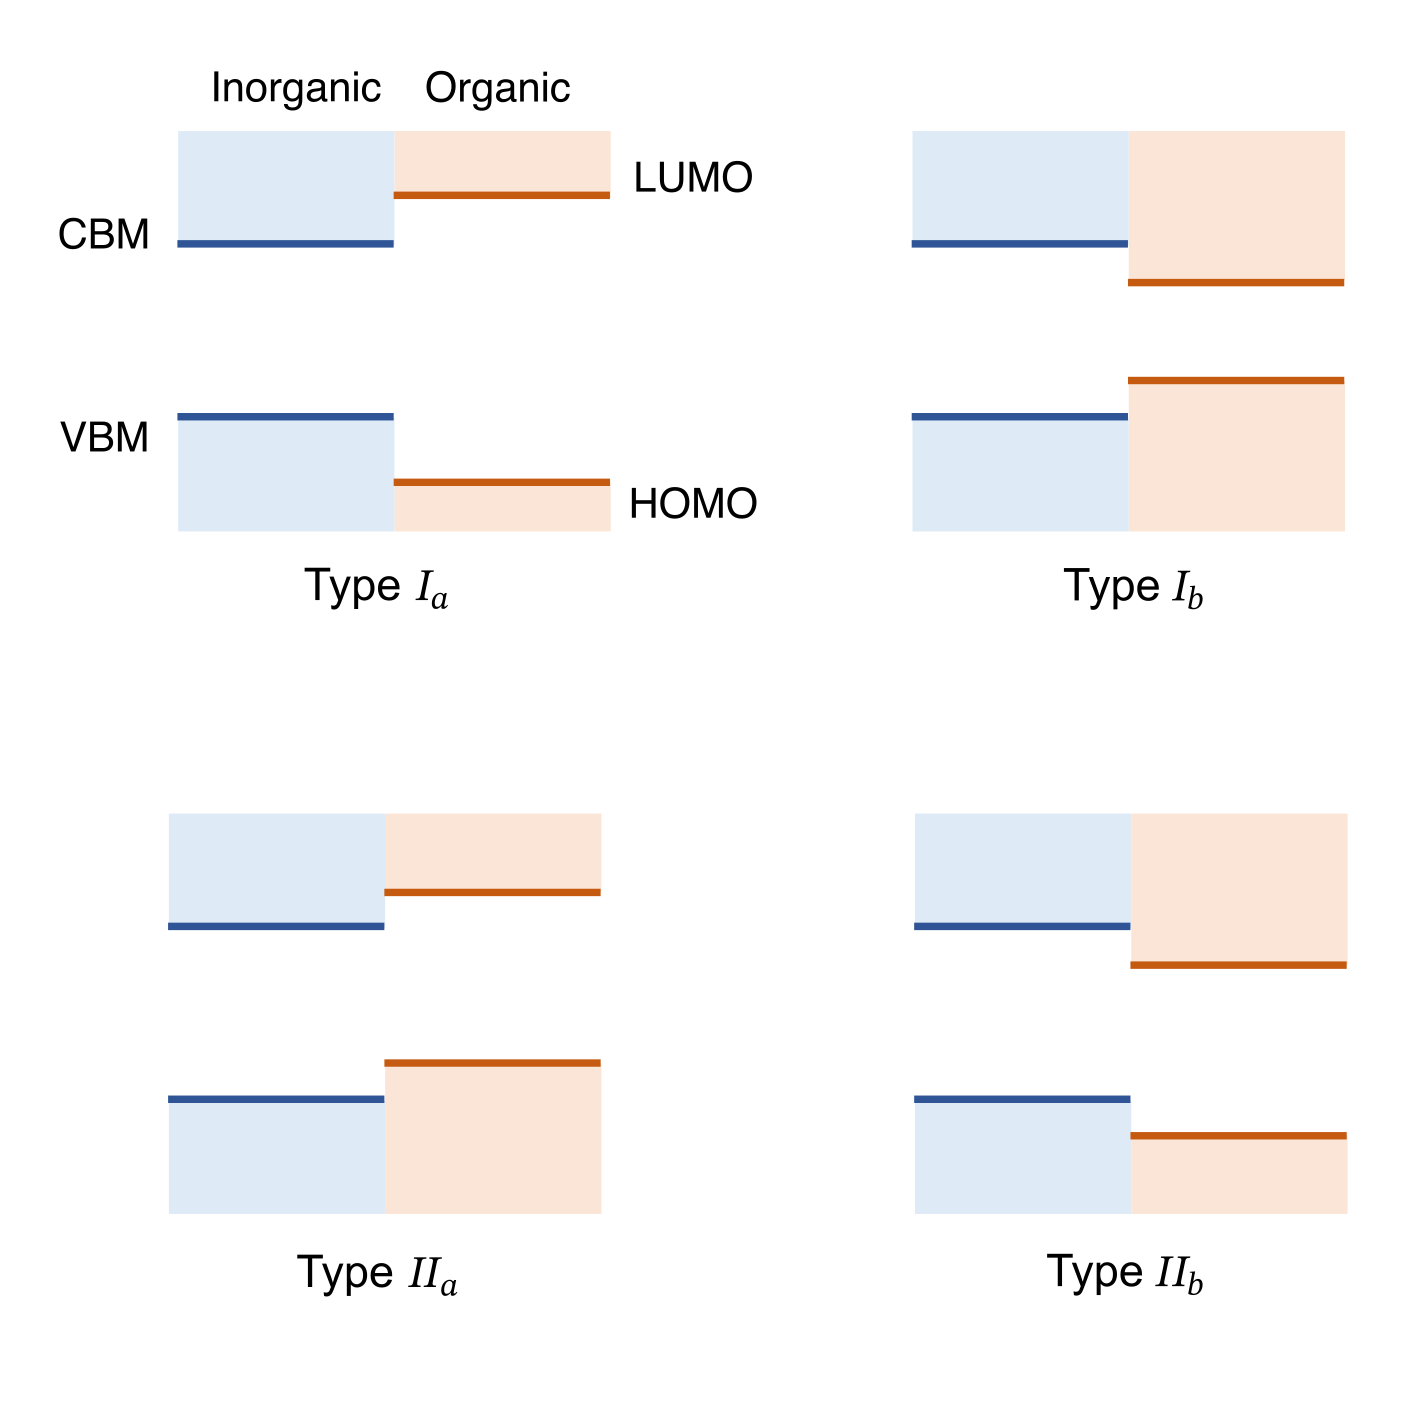
\includegraphics[width=0.6\textwidth]{figures/methodology/figure3-2.png}
    \caption{Schematic representation of energy level alignment types in 2D perovskites. }
    \label{fig:figure3.2}
\end{figure}

The classification of the energy level alignment types is shown in Figure \ref{fig:figure3.2}. In type I alignment, both low-energy electrons and holes are localized in the same component: type Ia in the inorganic layers and type Ib in the organic layers. In type II alignments, electrons and holes are separated between different components: in type IIa, electrons are localized in the inorganic layers and holes in the organic layers, whereas in type IIb, the reverse occurs. It should be noted that the designations “a” and “b” are sometimes interchanged in the literature depending on the component being emphasized\cite{RN18}. In other studies, only type I and type II are referenced without further categorization\cite{RN20}, and type Ib in our context is occasionally described as “reversed type I”\cite{RN606}. Notably, alignment type Ia is referred to as type Ib in some literature\cite{RN104,RN18}; here, we defined type Ia as the configuration where inorganic states serving as the band edges.

While the components of this workflow—database generation, high-throughput calculations, machine learning, and DFT validation—are common to AI-assisted materials discovery\cite{RN321,RN553}, the distinctive feature here is the integration of an invertible materials representation. Invertibility is a key attribute for materials representations in inverse design\cite{RN361}, ensuring two-way conversion between molecular structure and their representation. This type of invertible representation has been applied to some materials systems\cite{RN412,RN354}, but this is the first implementation in the context of hybrid materials. The absence of a versatile scheme of organic spacer representation has confined 2D perovskite research to forward design approaches, limiting the exploration of available chemical space. As we will show in this thesis, the workflow developed herein overcomes these limitations, facilitating the energy level alignment prediction. In addition, we expect that this fingerprint-based workflow will be generalized to investigate the correlation of other material properties with organic motifs in a wide range of hybrid material systems. 

\section{Invertible Molecular Fingerprints}\label{section:section3-2}

\begin{figure}[ht]
    \centering
    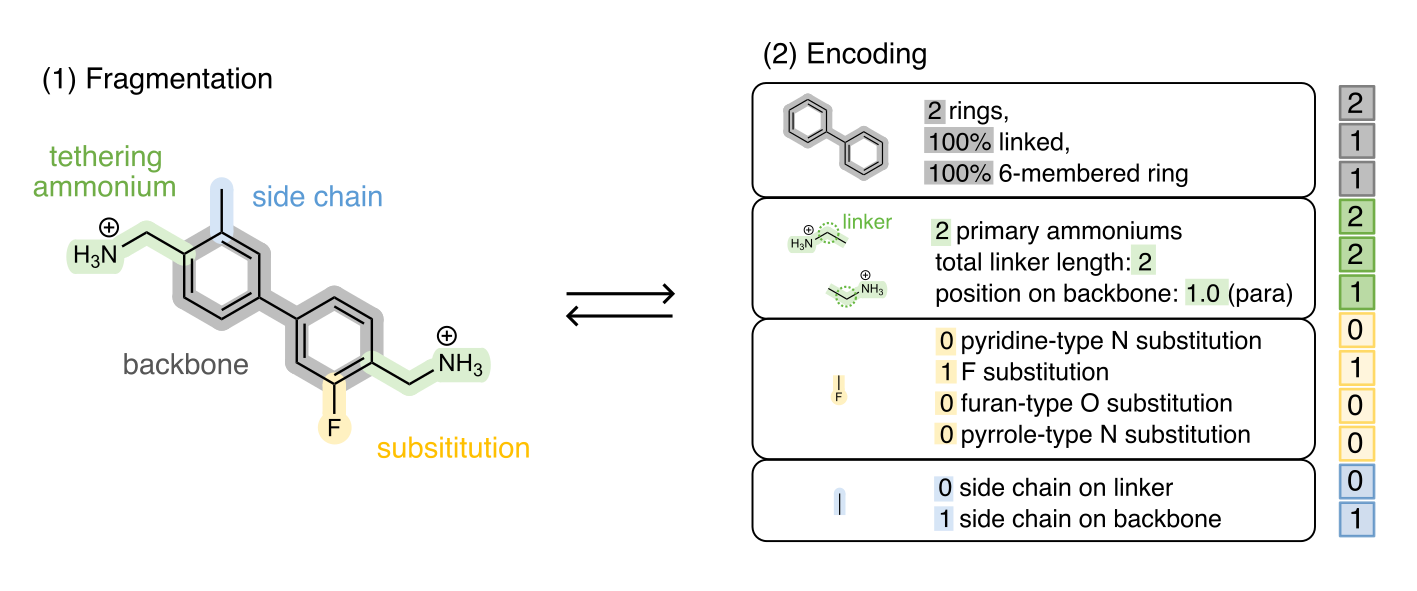
\includegraphics[width=\textwidth]{figures/methodology/figure3-3.png}
    \caption{Invertible molecular fingerprint representation for organic spacers in DJ perovskites.}
    \label{fig:figure3.3}
\end{figure}

Figure \ref{fig:figure3.3} depicts an overview of our fingerprinting scheme, which is based on the specific attributes of conjugated organic cations in 2D DJ perovskites, comprising two key components: molecular fragmentation and functional group encoding. Organic spacers are first fragmented into their building blocks (backbone, tethering ammonium, side chain, and substitutions) and then these building blocks are further encoded into a 12-digit fingerprint. 

\textbf{Fragmentation}

\begin{figure}[htbp]
    \centering
    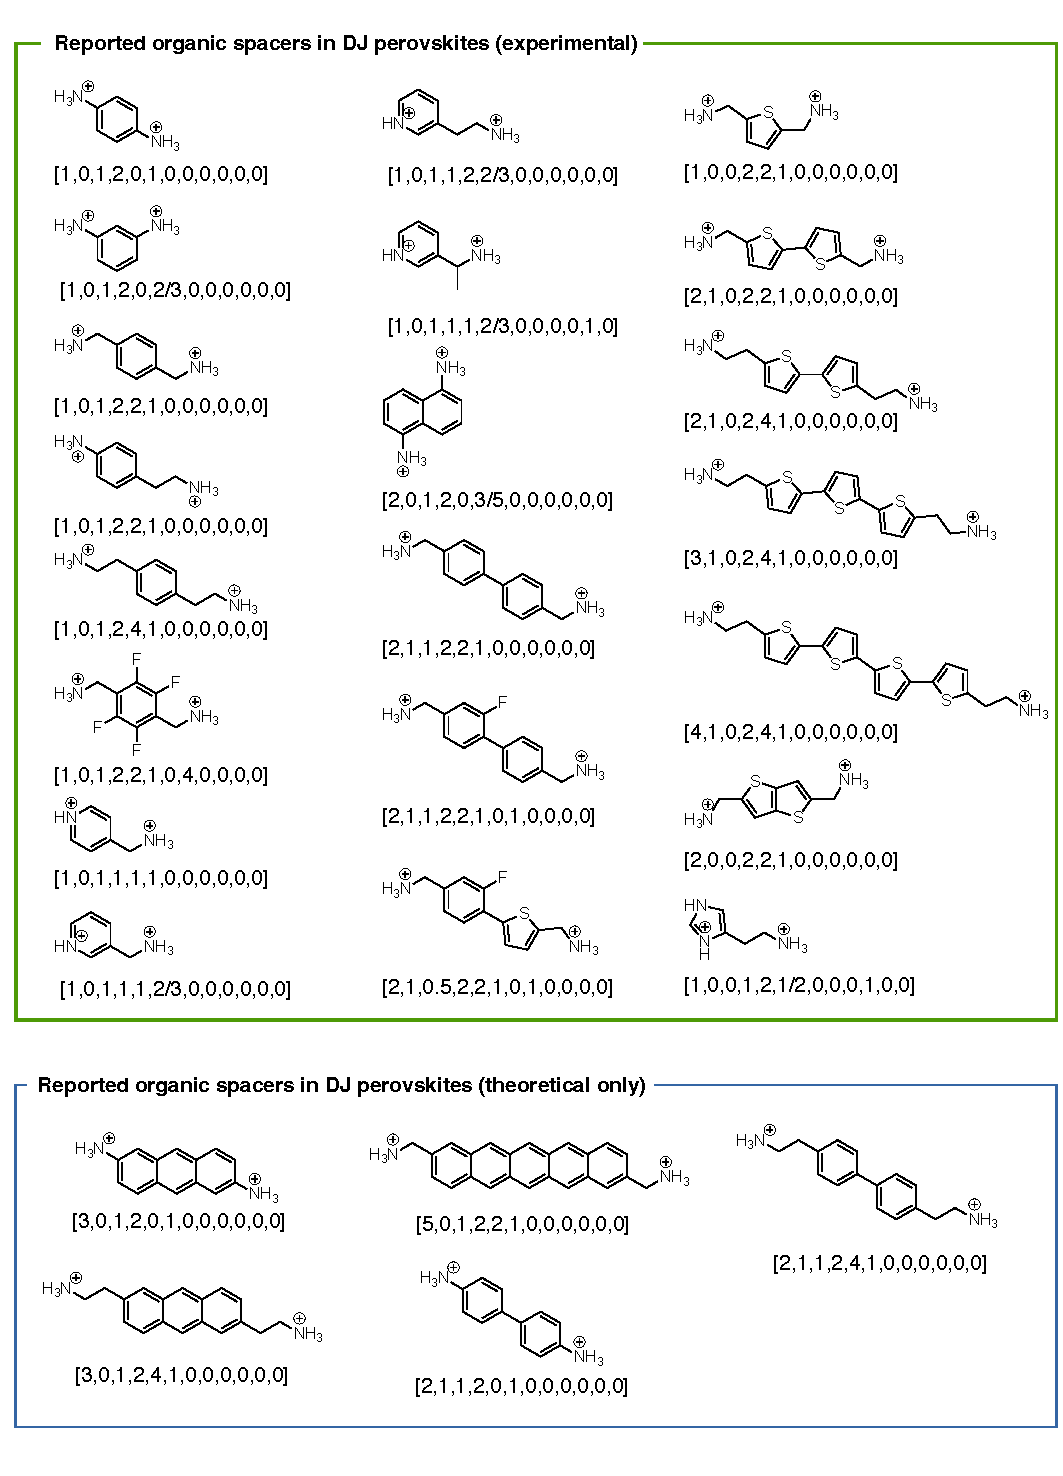
\includegraphics[width=\textwidth]{figures/methodology/figure3-4.pdf}
    \caption{Reported organic spacers included in this study with their molecular fingerprint.}
    \label{fig:figure3.4}
\end{figure}

\begin{figure}[htbp]
    \centering
    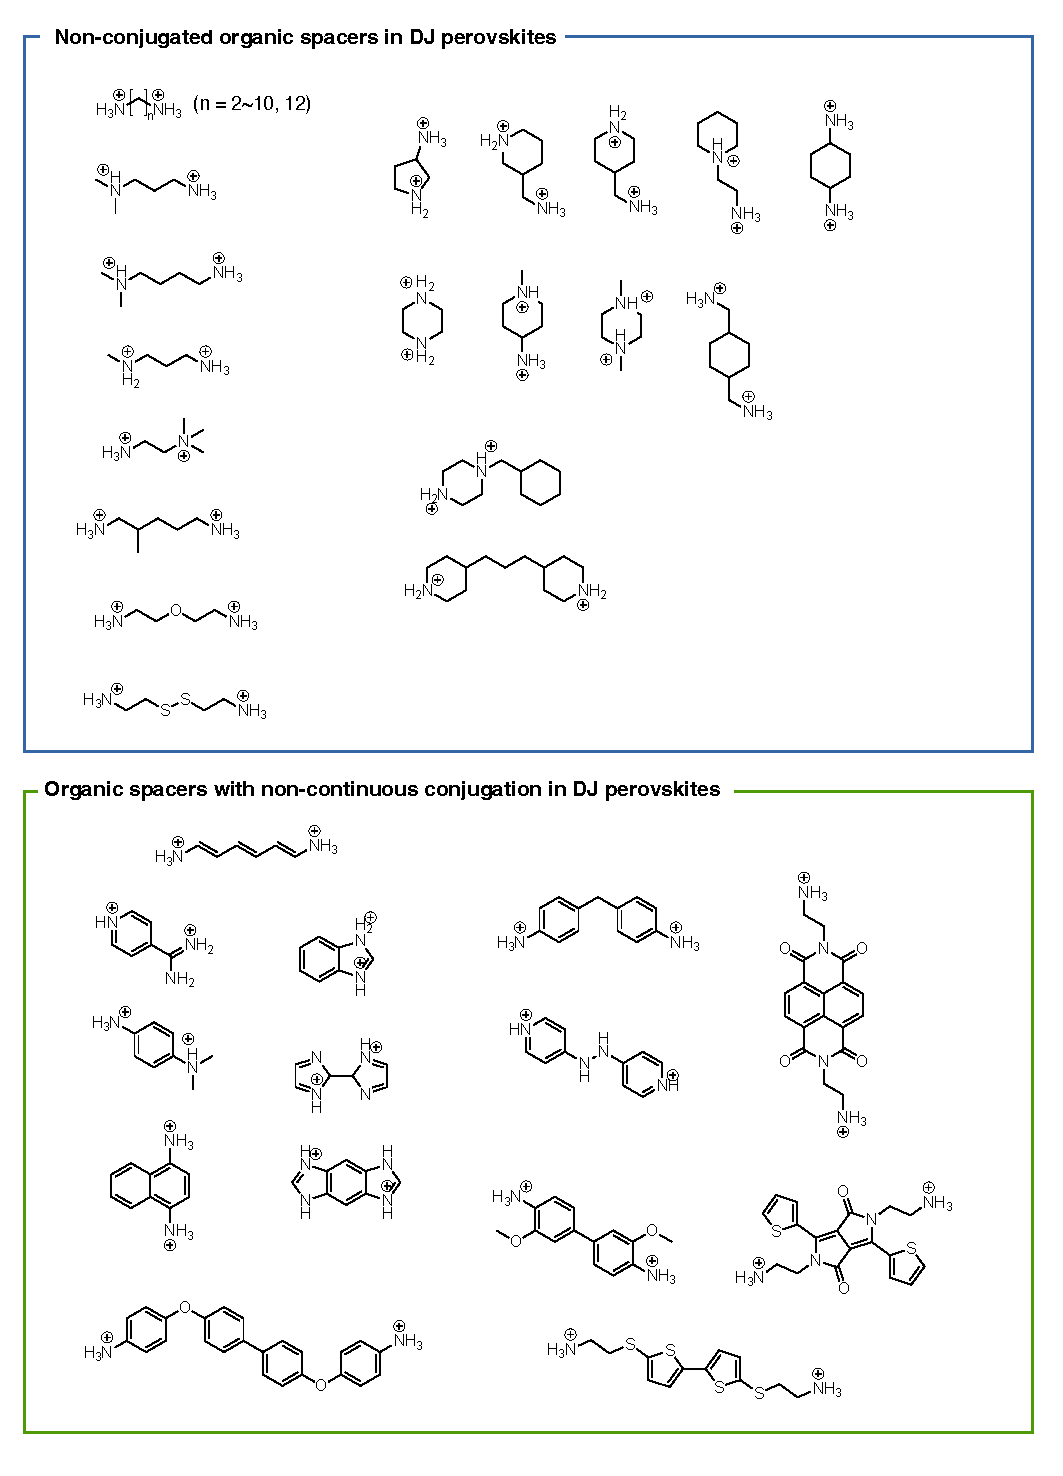
\includegraphics[width=\textwidth]{figures/methodology/figure3-5.pdf}
    \caption{Organic spacers excluded from the scope of this study.}
    \label{fig:figure3.5}
\end{figure}

The fragmentation is designed considering the structural motifs shared by reported conjugated diammonium spacers, as shown in Figure \ref{fig:figure3.4}. The DJ-phase organic spacers explored in this work are assumed to consist of four fragments: 

(1) a conjugated backbone of aromatic rings; 

(2) two tethering ammonium groups that anchor the spacer to the inorganic framework; 

(3) optional heteroatom substitutions;

(4) optional side chains. 

In this work, we limit the heteroatom substitutions to fluorine (F), oxygen (O), and nitrogen (N) on aromatic rings (benzene and thiophene). This simplification is based on two primary considerations: (1) their widespread use in semiconducting organic spacers within 2D perovskite systems, and (2) the need to preserve a chemically interpretable and synthetically accessible design space. Although including additional heteroatoms such as chlorine (Cl), bromine (Br), or phosphorus (P) could enhance electronic diversity, doing so would substantially expand the chemical space, increase fingerprint complexity, and introduce greater uncertainty in terms of synthetic feasibility and structural compatibility with the perovskite lattice.

These structural constraints significantly narrow the chemical space from a potentially immense size (estimated at $\sim10^{60}$ molecules for small organic molecules, as recognized in the context of drug discovery\cite{RN458}) to a much smaller subspace of organic spacers. 

We should note that the resulting chemical space is not exhaustive, leaving out some spacers, for example ones with alkyl backbones or non-continuous conjugation (Figure \ref{fig:figure3.5}). This fingerprinting scheme leads to a chemically relevant and computationally manageable set of organic cations (vide infra), giving rise to 2D DJ perovskite candidates with tailored properties. We primarily focused on semiconducting $\pi$-conjugated molecules due to their high relevance to optoelectronic applications of 2D perovskites and rich chemical diversity.

\textbf{Encoding}

\begin{figure}[ht]
    \centering
    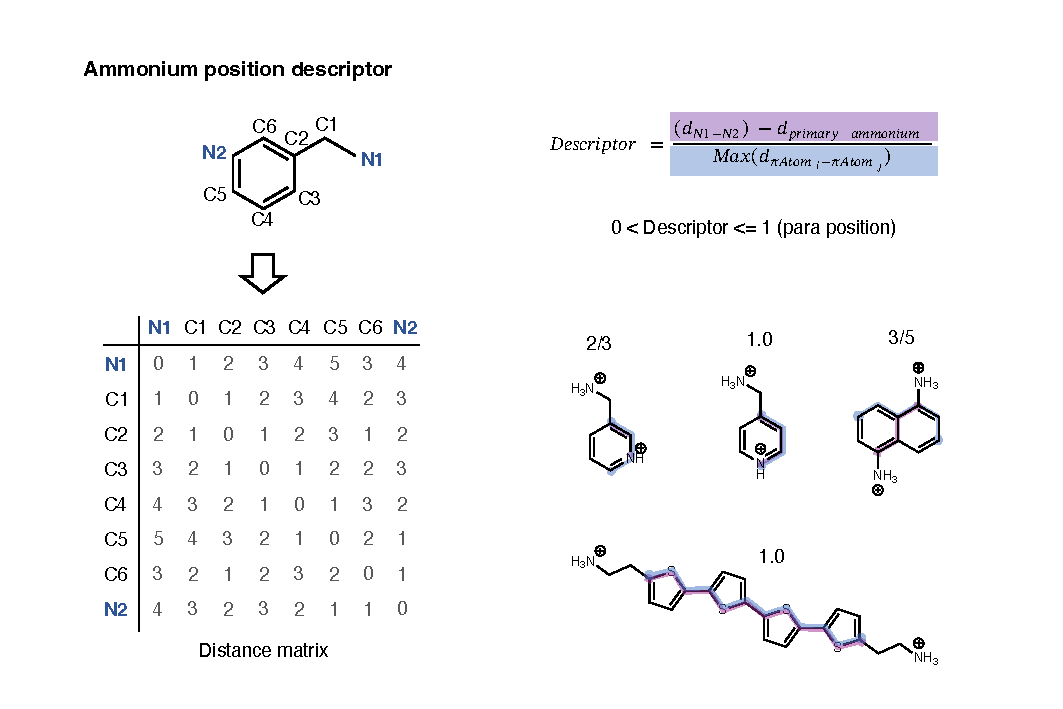
\includegraphics[width=\textwidth]{figures/methodology/figure3-6.pdf}
    \caption{Illustration of the ammonium position descriptor.}
    \label{fig:figure3.6}
\end{figure}

The encoding component of the scheme translates molecular structure into a fingerprint vector containing 12 customized descriptors, each representing a specific structural feature. Eleven descriptors are obtained by counting functional groups, while a unique “ammonium position” descriptor is derived from a distance matrix (Figure \ref{fig:figure3.6}). The main principle is to choose a minimal number of descriptors to reduce computational cost while these descriptors must be sufficient to describe the organic spacers relevant to DJ perovskites. As we will show later in the ML results in Chapter \ref{c:result-1}, there is minimal overlap between the descriptors, and they capture essential features for energy level prediction. 

For high-throughput purposes, all organic spacer structures in this study were stored in the Simplified Molecular Input Line Entry System (SMILES) format, a widely used textual representation of molecular structure. Molecular fingerprinting was performed to extract key structural and chemical descriptors automatically using the RDKit library in Python. The workflow took the SMILES representation of the organic spacer as input and returned a set of 12 organic descriptors, categorized as follows:

\begin{enumerate}
    \item Conjugated backbone descriptors: number of rings; percentage of ring linkages; percentage of six-membered rings
    \item Tethering ammonium descriptors: number of primary ammonium groups ($NH_3^+$); linker length (distance between ammonium groups and backbone); and ammonium position on the backbone
    \item Heteroatom substitution descriptors: number of nitrogen atoms (pyridine-type); number of fluorine atoms, number of oxygen atoms (furan-type); number of nitrogen atoms (pyrrole-type)
    \item Side chain descriptors: number of side chain attached to linkers; number of side chains attached to the backbone 
    
\end{enumerate}

Descriptors were computed using SMARTS (SMiles ARbitrary Target Specification) patterns, enabling the identification and counting of specific functional groups. A new descriptor, the ammonium position on the backbone, was developed specifically for this work. This descriptor quantifies the relative position of tethering ammonium groups on the conjugated backbone using a distance matrix approach, as depicted in Figure \ref{fig:figure3.6}.

The ammonium position descriptor is derived from the molecular skeleton using a distance matrix. This descriptor is calculated as the ratio of the maximum distance along the conjugated backbone to the distance between the tethering ammonium group and the backbone. Representative organic spacers with their corresponding ammonium position descriptors are shown in Figure \ref{fig:figure3.6}.

We should note that the molecule-fingerprint correspondence is not exclusive, in other words, some molecular isomers share the same fingerprint. Although additional descriptors, or longer fingerprints (e.g., heteroatom substitution position, and side chain position) could offer more structural detail, we found such features have minimal impact on electronic properties, making the current fingerprinting scheme sufficient for predicting new DJ perovskites with all four band alignment types.

\begin{figure}[ht]
    \centering
    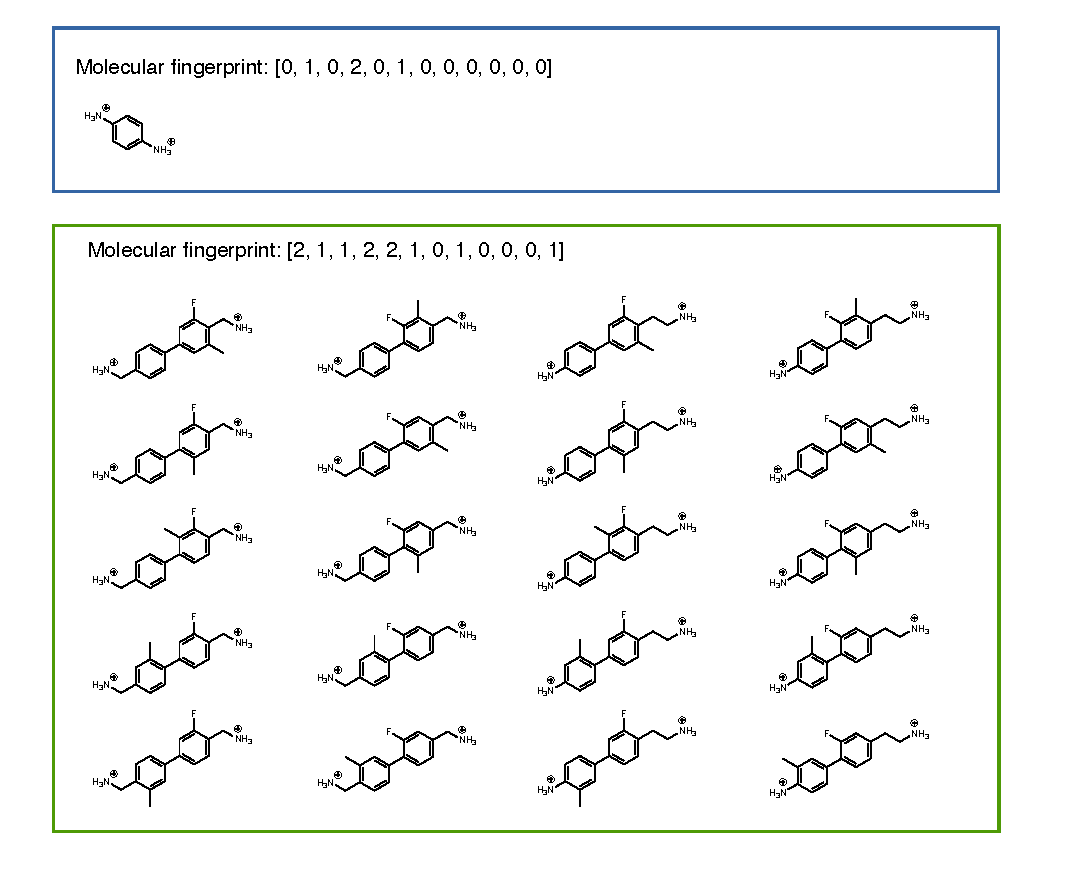
\includegraphics[width=\textwidth]{figures/methodology/figure3-7.pdf}
    \caption{An illustration of one-to-one (top) and one-to-multiple (bottom) mappings between a molecular fingerprint and its corresponding organic spacer(s).}
    \label{fig:figure3.7}
\end{figure}

Figure \ref{fig:figure3.7} illustrates the relationship between a fingerprint and its corresponding organic spacer(s). The upper panel shows a one-to-one mapping, where a fingerprint corresponds to a single organic spacer. In contrast, the lower panel shows a one-to-many mapping, where multiple organic spacers (isomers) share the same fingerprint, including the example shown in Figure \ref{fig:figure3.3}. These isomers may differ in structural features such as the position of heteroatom substitution, side chain placement, or the linker length between tethering ammonium groups. While such variations may affect to a certain extent the chemical and physical properties of the cations, the the energy levels are almost the same due to the shared molecular backbone. However, these isomers may have different levels of synthesis feasibility, which warrants elucidation based on future detailed analysis and experimental efforts. At this stage, no additional screening is applied to these isomers. All molecules corresponding to a given fingerprint are retained in the dataset to preserve the full chemical diversity for downstream analysis.

In previous AI-assisted 2D perovskite discovery efforts, organic spacers are typically represented using physiochemical descriptors\cite{RN315,RN283}, but an effective molecular representation scheme that can explicitly capture the molecular structure has not been established. In the myriad research fields involving organic molecules, the structural variations are often encoded using digits (e.g., fingerprints), strings (e.g., SMILES), or graph-based methods\cite{RN361}. Among these, fingerprinting methods—such as the widely adopted but non-invertible 2048-digit Morgan fingerprint—have demonstrated their efficiency in AI-assisted workflow\cite{RN610,RN549}. In contrast, our 12-digit fingerprint scheme has been tailored according to the specific attributes of 2D hybrid perovskites, offering several advantages. First, it is efficient, with minimal redundancy and overlap between descriptors, ensuring a compact representation that captures structural variation most relevant to DJ perovskites. Second, it is interpretable, enabling human experts to extract meaningful insights into the encoded structural variations. Finally, it is invertible, allowing direct mapping back to the molecular structure by both human experts and machines, which is essential for inverse design.

\section{High-throughput calculation}\label{section:section3-3}

\textbf{Molecular morphing}

Molecular morphing was implemented as a systematic method to explore chemical space by generating variants of molecular structure. The process used reaction SMARTS patterns implemented in the RDKit library to iteratively apply predefined chemical transformations. This approach performs stepwise modifications on a starting molecular structure, generating new variants while adhering to defined chemical constraints. 

\begin{figure}[ht]
    \centering
    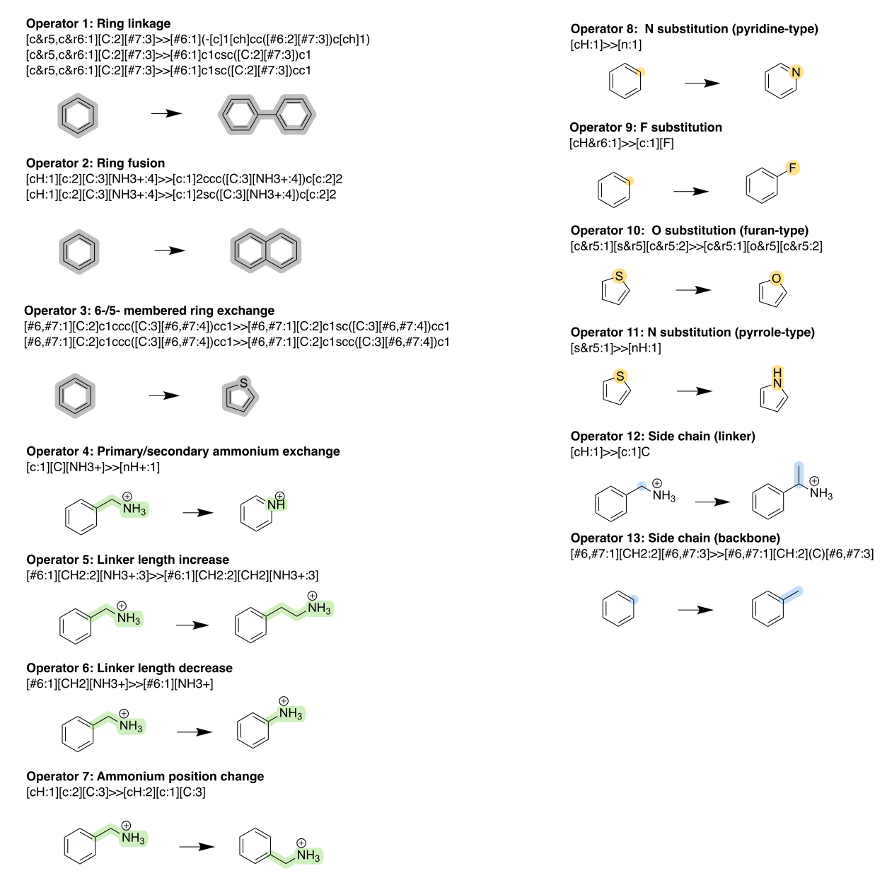
\includegraphics[width=0.9\textwidth]{figures/methodology/figure3-9.png}
    \caption{List of molecular morphing operators used in this study for generation of hypothetical organic spacers.}
    \label{fig:figure3.8}
\end{figure}

The molecular morphing process began with  PDMA, a well-characterized prototype molecule, represented in SMILES format. As shown in Figure \ref{fig:figure3.8}, a set of 13 morphing operators, encoded as 17 unique SMARTS patterns, was defined to ensure that each transformation adhered to established chemical constraints. These morphing operation include:
increasing number of rings, substituting heteroatoms on aromatic rings, modifying linker lengths, etc.

Each operator was applied iteratively to the starting molecule to generate new molecular structures. The newly generated molecules were stored as SMILES strings, ensuring compatibility with downstream fingerprinting and modelling workflows.

PDMA was chosen as the starting molecule due to its structural simplicity and extensive study in the literature. Figure \ref{fig:figure3.9} illustrates the distribution of existing spacers across generations when different candidates are selected as $G_0$ molecules. PDMA (top right) was selected because it results in most existing spacers appearing in early generations, demonstrating its structural simplicity and suitability for easy transformation into other molecular structures via morphing operations.


\begin{figure}[ht]
    \centering
    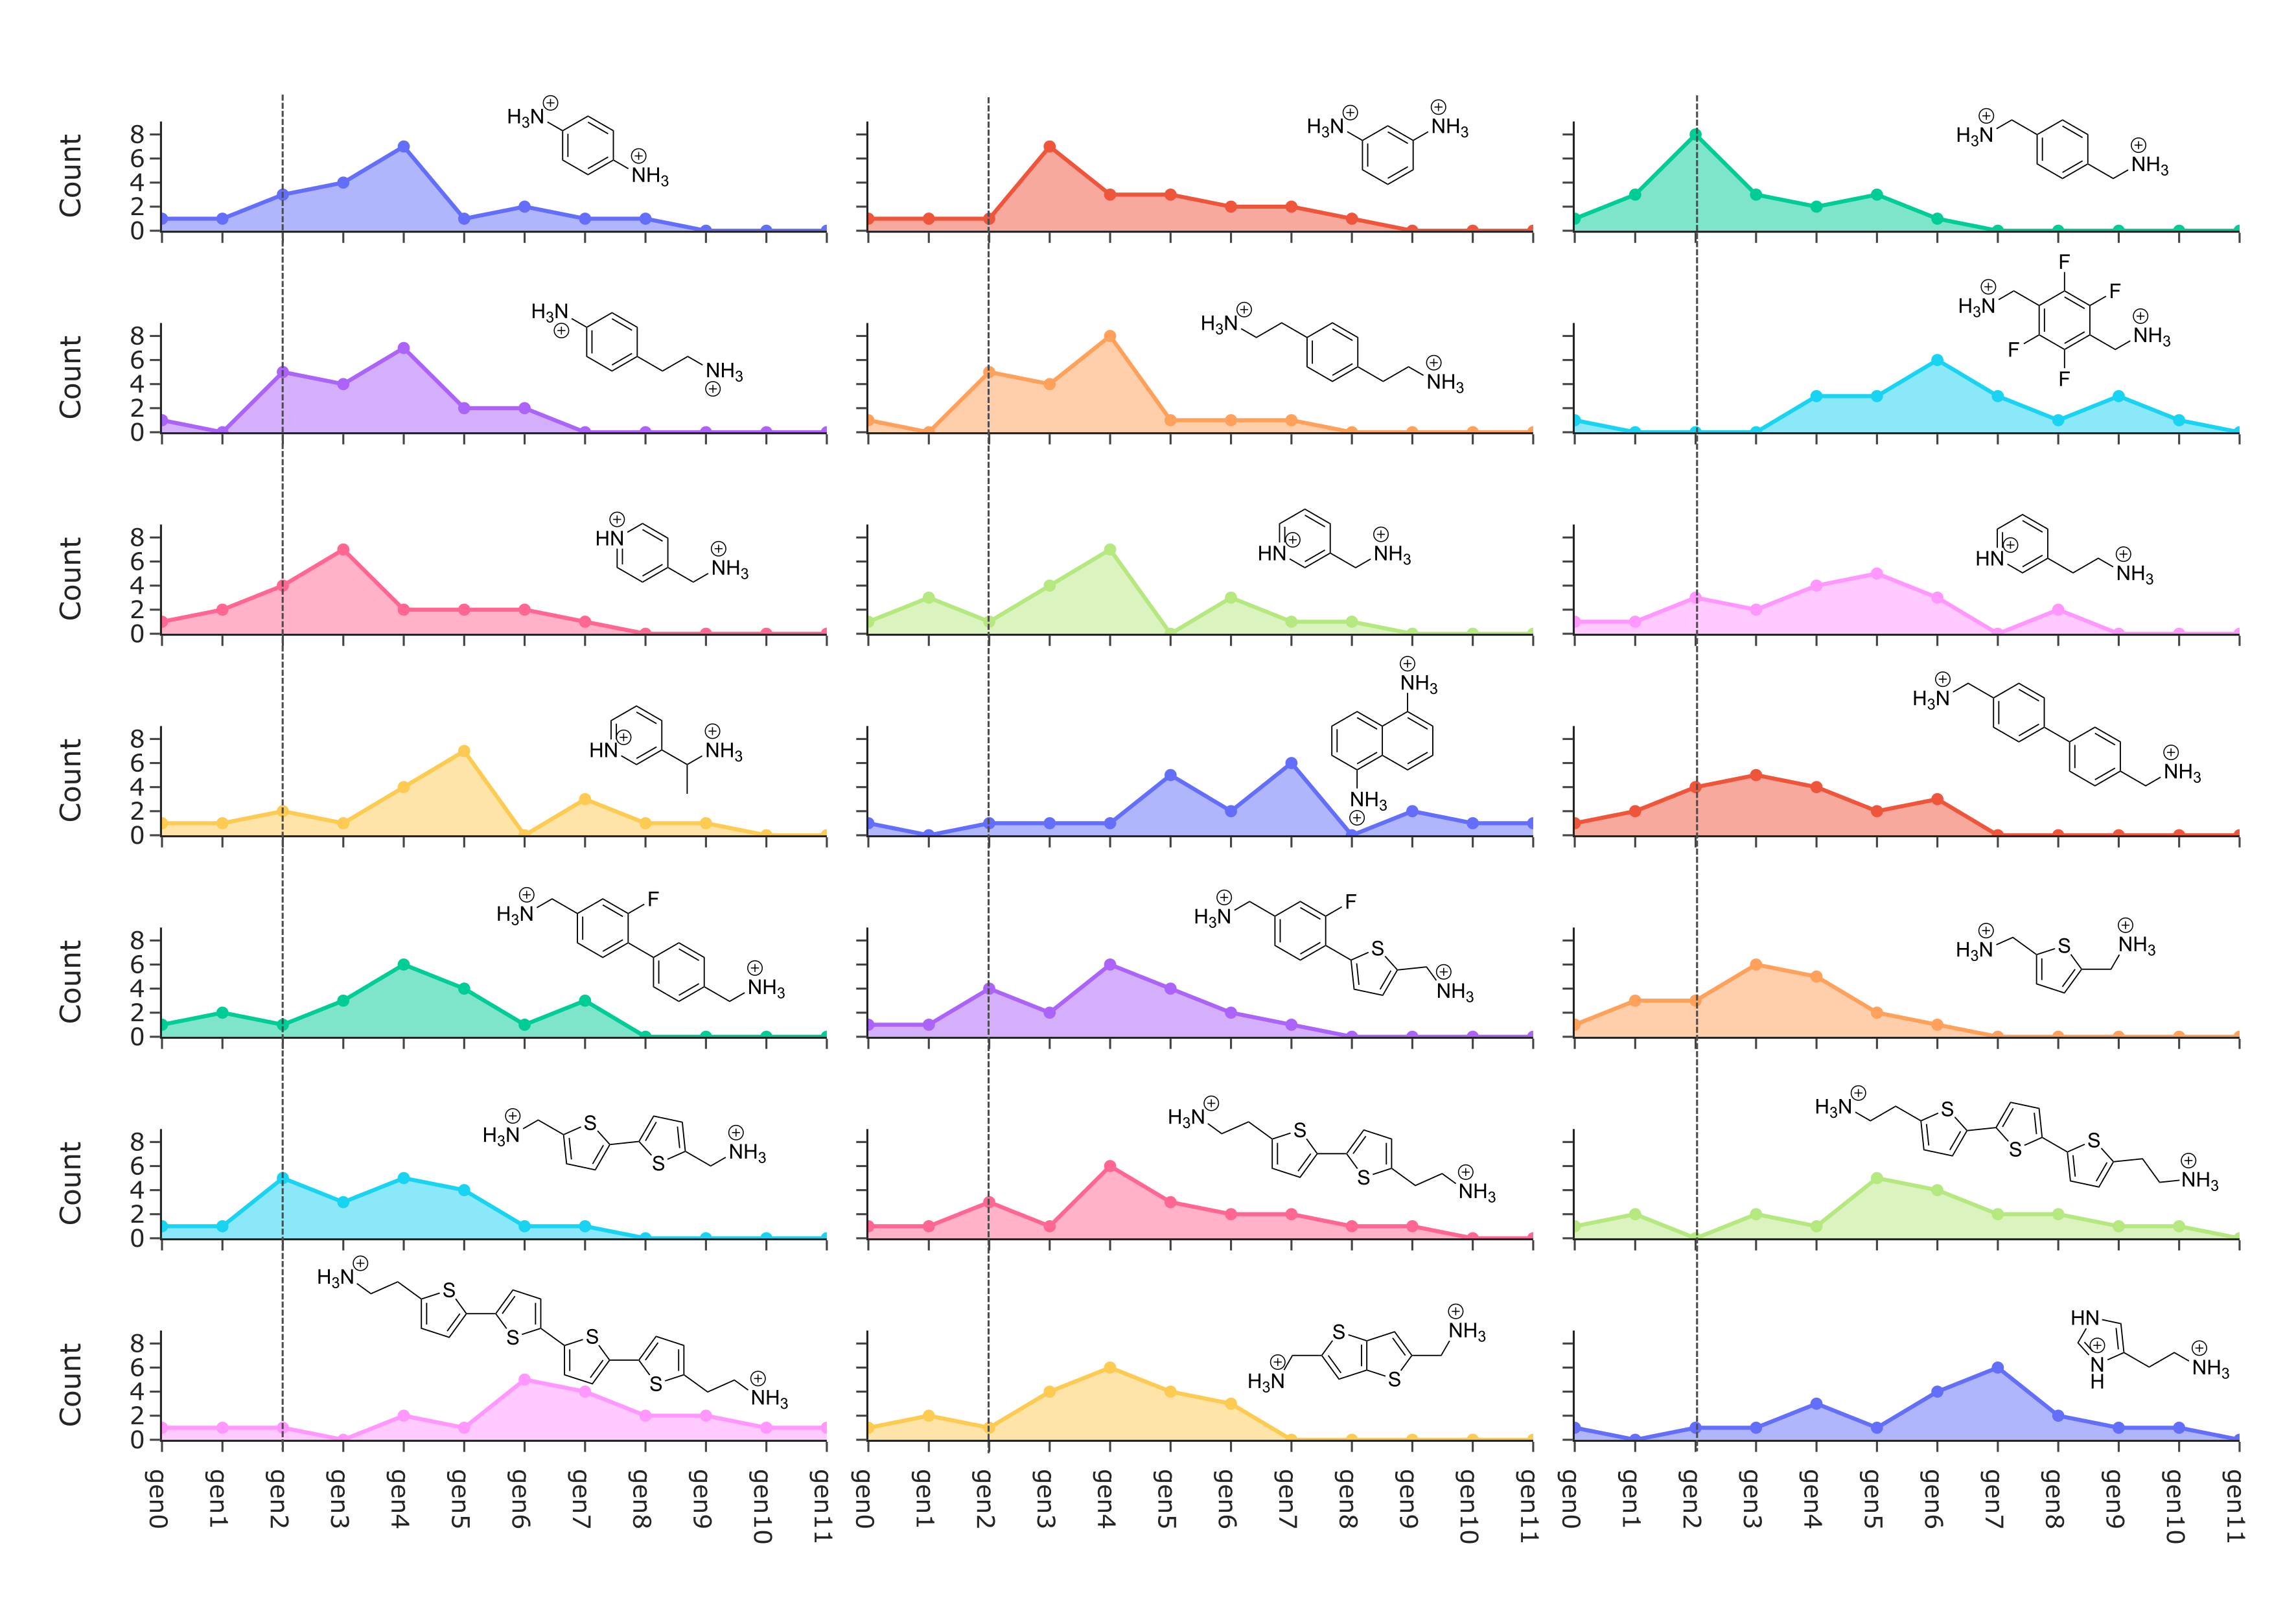
\includegraphics[width=\textwidth]{figures/methodology/figure3-8.png}
    \caption{Rationale for selection of PDMA as the generation $G_0$ organic spacer.}
    \label{fig:figure3.9}
\end{figure}


\textbf{Frontier level calculation of organic spacers}

The 3D molecular structures of organic spacers were generated from SMILES string using the RDKit library, which efficiently converts the molecular graph representations into 3D coordinates. Conformational sampling was conducted assuming the isolated, gas-phase configurations of the spacers, independent of their incorporation into the 2D perovskite structure. 

DFT calculations were performed using Gaussian 09 package with the B3LYP functional and 6-31G** basis set to calculate the energy levels of the HOMO and LUMO.

\textbf{Hybrid Perovskite Structure Generation}

The hybrid perovskite structures were constructed by inserting the organic spacers into a PbI$_4$-based inorganic framework. Initial conformations of the organic spacers were visualized in Avogadro and adjusted according to literature-reported configurations to reflect their likely conformations within the 2D perovskites. Specific modifications include: 

(1) Ensuring the linearity of linker groups to reduce aggregation effects observed in isolated forms. 

(2) Constraining rotations of linked aromatic rings to reflect dihedral angles typically found in hybrid perovskites, which are smaller than those in the isolated gas phase. For instance, benzene-benzene linkages were assigned a dihedral angle of 20°; thiophene-thiophene and thiophene-benzene linkages were constrained to 0°.

A $2\times2\times1$ supercell of PbI$_6$ octahedra was employed (each unit cell containing four organic spacers and four PbI$_4$ units), starting with an ideal cubic configuration in inorganic layers. Organic spacers are aligned along the lattice c direction, with two ammonium tethering groups intercalated within the cavities formed by the PbI$_6$ octahedra. Organic spacers are arranged in herringbone (out-of-phase) configuration. This configuration was chosen as it is frequently observed in experimental studies, with minimal influence on the electronic structure compared to other configurations. Interlayer distances between neighbouring PbI$_4$ layers were modulated according to spacer length, ensuring realistic structural representation. The framework was built programmatically using a combination of RDKit and pymatgen.

\begin{figure}[ht]
    \centering
    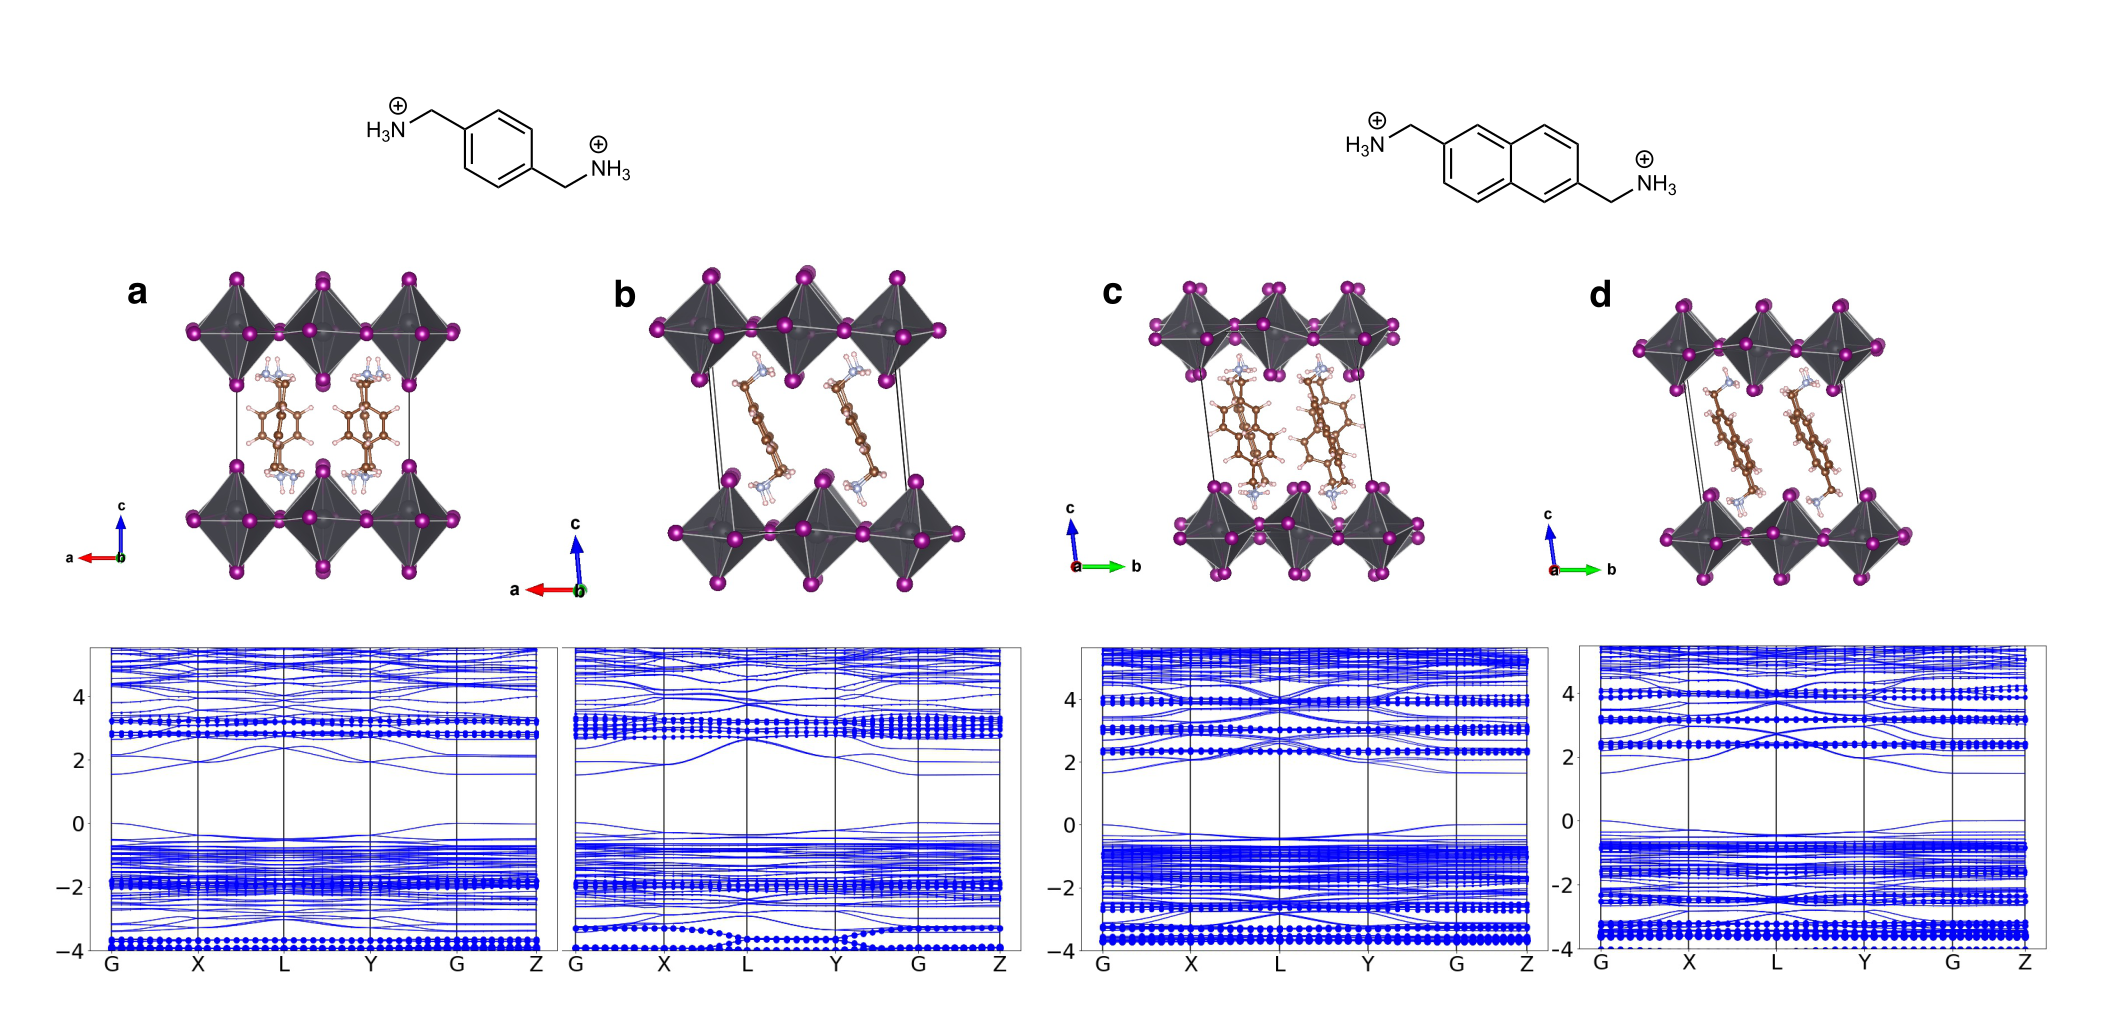
\includegraphics[width=\textwidth]{figures/methodology/figure3-10.png}
    \caption[Crystal structures and band structures of DJ perovskites with different organic spacer packing arrangements.]{Crystal structures and band structures of DJ perovskites with different organic spacer packing arrangements. Two example spacers are shown. Panels \textbf{a} and \textbf{c} illustrate out-of-phase (herringbone) packing, while \textbf{b} and \textbf{d} show in-phase packing.}
    \label{fig:figure3.10}
\end{figure}

Figure \ref{fig:figure3.10} shows a comparison between different packing pattern of organic spacers and their influence on the energy level in 2D perovskites. Figure \ref{fig:figure3.10}a and c shows the out-of-phase (herringbone) arrangement of organic spacers. This configuration is commonly observed in reported 2D perovskites, and our DFT calculation indicate this type of packing leads to minimal dispersion of molecular orbitals. Figure \ref{fig:figure3.10}b and d shows the in-phase arrangement, a configuration typically found in oligomer thiophene-based spacers. Our DFT calculation indicate that the molecular orbitals exhibit sizable dispersion ($\sim0.7$ eV as observed in this study), consistent with previous reports attributing this behaviour to electronic coupling among tightly packed adjacent organic spacers\cite{RN2}. Notably, one study indicates that out-of-phase configurations are energetically favoured\cite{RN41}. For consistency, we adopt the out-of-phase packing pattern across all structures. We anticipate that this in-plane dispersion of molecular orbitals will not affect our proposed final candidates for energy level alignment type Ib, IIa, and IIb, as this dispersion primarily broadens the organic frontier levels without shifting their centres.

\textbf{Perovskite Structure Relaxation}

DFT-based structure relaxations were performed using the Vienna Ab initio Simulation Package (VASP) with the Perdew-Burke-Ernzerhof (PBE) functional and projector augmented wave (PAW) pseudopotentials. Grimme’s DFT-D3 dispersion correction with zero damping was included to account for van der Waals interactions critical to layered perovskites. Relaxation was conducted in two steps: 

(1) A preliminary relaxation with a loose reciprocal density of 64 (resulting in k-point grids such as $1\times1\times1$ or $1\times1\times2$, depending on the lattice parameters along the c-axis). 

(2) A tighter relaxation with a reciprocal density of 300 (resulting in k-point grids such as $3\times3\times2$, $3\times3\times3$, or $3\times3\times4$). Convergence criteria required an energy difference per atom below $5\times10^{-6}$ eV.

\textbf{Electronic Structure Calculations}



To investigate the electronic properties of 2D perovskites, spin-orbit coupling (SOC) was included due to the significant relativistic effects in Pb-based compounds. The following workflow addressed the known limitations of commonly used functionals in predicting bandgap values and ensure alignment with experimental data: 

\begin{enumerate}
    \item Band structure shape identification: The band structure across the Brillouin zone was initially calculated using the PBE+SOC functional. This functional effectively captures the qualitative shape of the band structure but is known to underestimate the bandgap for perovskite materials. The results provided a foundational map of the electronic band dispersion. 

    \item Accurate bandgap calculation at representative points: To obtain accurate bandgap values, the HSE06+SOC hybrid functional was applied at critical points in the Brillouin zone ($\Gamma$ and Z). This method corrects the bandgap underestimation of PBE+SOC, ensuring quantitative agreement with experimental values. For structures with interlayer distances below 5 $\AA$, calculations were performed at both $\Gamma$ and Z points to capture the dispersion of inorganic bands from $\Gamma$ to Z. For larger interlayer distances (greater than 5 $\AA$), calculations were focused on the $\Gamma$ point only, as the dispersion becomes negligible. A Hartree-Fock exchange (HF) percentage of 40\% was used in the HSE06+SOC calculations, yielding bandgap values with a deviation of only 0.05 eV from experimental results. 

\begin{figure}[ht]
    \centering
    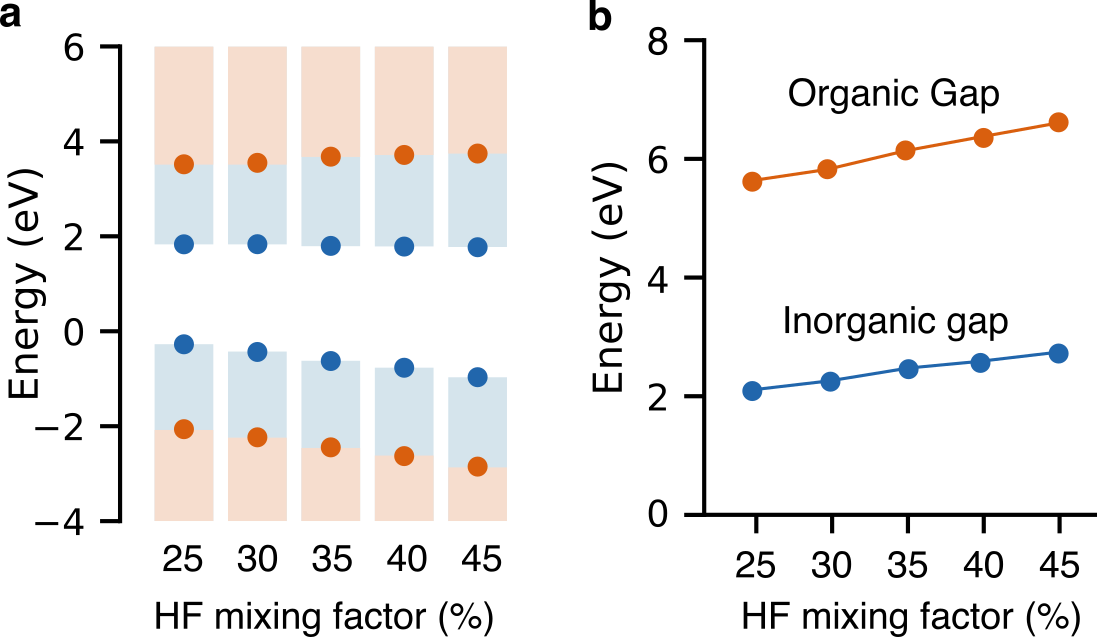
\includegraphics[width=0.75\textwidth]{figures/methodology/figure3-11.png}
    \caption[Effect of Hartree–Fock (HF) mixing factor on the calculated energy levels of organic and inorganic components in DJ-phase perovskites with the G$_0$ molecule (PDMA).]{Effect of Hartree–Fock (HF) mixing factor on the calculated energy levels of organic and inorganic components in DJ-phase perovskites with the G$_0$ molecule (PDMA). \textbf{a} Variation in energy level alignment with increasing HF mixing. \textbf{b} Evolution of the organic and inorganic energy gaps as a function of HF mixing factor.}
    \label{fig:figure3.11}
\end{figure}

\begin{figure}[ht]
    \centering
    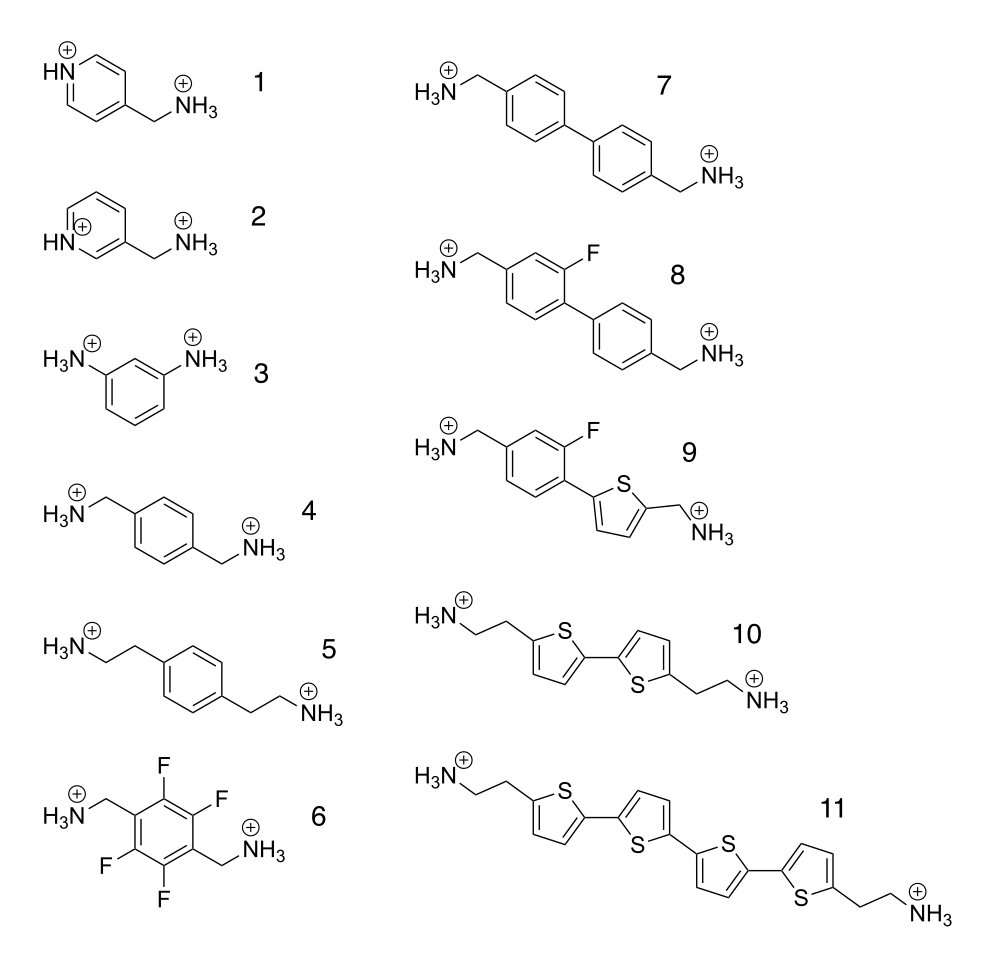
\includegraphics[width=0.6\textwidth]{figures/methodology/figure3-12.png}
    \caption{Reported organic spacers for which experimental bandgap values have been measured in the corresponding DJ perovskites.}
    \label{fig:figure3.12}
\end{figure}

\begin{table}[!ht]
    \centering
    \caption[Comparison of bandgap values calculated using HSE + SOC, HF=40\% and reported experimental values.]{Comparison of bandgap values calculated using HSE + SOC, HF=40\% and reported experimental values. Compound IDs correspond to the organic spacers listed in Figure \ref{fig:figure3.12}.}\label{table:table3.1}
    \begin{tabular}{|l|l|l|}
        \hline
        \textbf{Compound} & \textbf{Calculation (eV)} & \textbf{Experiment (eV)} \\  \hline
        1 & 2.42 & -\cite{RN31} \\ \hline
        2 & 2.26 & 2.34\cite{RN31} \\ \hline 
        3 & 2.39 & 2.42\cite{RN33} \\ \hline
        4 & 2.56 & 2.44\cite{RN86}, 2.42\cite{RN34} \\ \hline 
        5 & 2.42 & 2.46\cite{RN86}, 2.43\cite{RN95} \\ \hline 
        6 & 2.57 & 2.58\cite{RN95} \\ \hline
        7 & 2.38 & 2.52\cite{RN84} \\  \hline
        8 & 2.56 & 2.42\cite{RN84} \\  \hline 
        9 & 2.56 & 2.39\cite{RN84} \\  \hline
        10 & 2.79 & -\cite{RN41} \\ \hline 
        11 & 2.38 & 2.38\cite{RN38} \\ \hline 
    \end{tabular}
\end{table}

\begin{table}[!ht]
    \centering
    \caption[Effect of HF mixing factor on the calculated bandgap values of DJ perovskites.]{Effect of HF mixing factor on the bandgap values of DJ perovskites. Compound IDs correspond to the organic spacers listed in Figure \ref{fig:figure3.12}.}
    \label{table:table3.2}
    \begin{tabular}{|l|l|l|}
        \hline
          & \textbf{Compound 2 (eV)} & \textbf{Compound 4 (eV)} \\ \hline
        \textbf{Experiment} & 2.34\cite{RN31} & 2.44\cite{RN86}, 2.42\cite{RN34} \\ \hline
        \textbf{25\%} & 1.82 & 2.12 \\ \hline
        \textbf{30\%} & 1.97 & 2.26 \\ \hline
        \textbf{35\%} & 2.11 & 2.41 \\ \hline
        \textbf{40\%} & 2.26 & 2.56 \\ \hline
        \textbf{45\%} & 2.42 & 2.71 \\ \hline
    \end{tabular}
\end{table}

    Figure \ref{fig:figure3.11} shows the impact of mixing factor on the organic frontier levels in DJ perovskite. A range of mixing factors (25\% to 45\%) has been employed in earlier studies to match experimental bandgap values. In this work, we select a mixing factor of 40\%, as it yields the smallest average error of 0.05 eV. The mixing factor impacts the organic levels slightly more than the inorganic levels, though both follow very similar trends. This suggests that the energy level alignment type is unlikely to vary significantly for most proposed DJ perovskites. 

    Table \ref{table:table3.1} and \ref{table:table3.2} shows the bandgap of several existing DJ perovskites with different mixing factors, confirming the mixing factor of 40\% yield the smallest error compared to experimental value.

    \item Refined band structure across the Brillouin zone: To extend the high accuracy of HSE06+SOC calculations across the entire Brillouin zone without incurring the prohibitive computational cost, a scissoring technique was applied. The band structure obtained from PBE+SOC was adjusted using the band edges calculated at the $\Gamma$ and Z points with HSE06+SOC. The scissoring operation aligned the PBE+SOC-derived band structure with the inorganic band edge and organic frontier orbital levels predicted by HSE06+SOC, providing a consistent, high-fidelity representation of the electronic structure.
\end{enumerate}



\textbf{High-throughput framework}

The high-throughput DFT calculations for both organic spacers and hybrid perovskite structures were conducted on the Gadi supercomputer, utilizing a workflow based on the Materials Project (MP) input parameter template. The MP standards are widely recognized as the minimal benchmark in the field of DFT calculations, ensuring reproducibility and consistency across studies. These parameters are particularly suitable for capturing the general structural and electronic properties of a wide range of materials.

To meet the specific demands of hybrid perovskite systems, which are characterized by strong spin-orbit coupling, van der Waals interactions, and low-symmetry structures, we further refined and tightened the computational parameters. Key refinements included:

\begin{itemize}
    \item Energy Convergence Criterion: The MP default for electronic energy convergence (EDIFF) is $5\times10^{-5}$ eV per calculation. For our study, we set a stricter threshold of $5\times10^{-6}$ eV per atom to ensure reliable energy differences for low-symmetry perovskite structures.
    \item Plane-Wave Cutoff Energy: While the MP standard cutoff energy is typically 520 eV, we adjusted this to 480 eV, as testing showed that this value-maintained accuracy for perovskite systems while optimizing computational efficiency.
    \item Reciprocal Space Sampling: For initial structural relaxation, we used the default MP reciprocal density of 64 (resulting in k-point grids such as $1\times1\times1$ or $1\times1\times2$, depending on the c-axis lattice parameter). For final relaxation and electronic property calculations, we increased the reciprocal density to 300, corresponding to dense k-point grids such as $3\times3\times3$, $3\times3\times2$, or $3\times3\times4$. This stricter k-point sampling ensured accurate modelling of structural distortions and electronic properties in the layered perovskites.
    \item Dispersion Corrections: To account for van der Waals interactions in layered systems, Grimme’s DFT-D3 dispersion correction with zero damping was included. This refinement is critical for accurately describing interlayer interactions in 2D perovskites.
\end{itemize}

The high-throughput framework was automated using the pymatgen library to generate VASP input files and parse outputs, enabling systematic and efficient exploration of $\sim3,000$ organic spacers and $\sim400$ hybrid perovskite structures. By building on the minimal standards established by the Materials Project and incorporating additional refinements specific to perovskites, we ensured that our computational results met the highest standards of accuracy and reliability for this material system.

\section{Machine Learning}\label{section:section3-4}

All machine learning tasks in this thesis were conducted using the Scikit-learn library in Python. This included data preprocessing, dimensionality reduction, training of regression and classification models, and extraction of feature coefficients for model interpretation.

\textbf{Dimensional reduction for chemical space visualization}

To visualize the chemical space of organic spacers, we employed unsupervised learning techniques for dimensionality reduction. We compared Principal Component Analysis (PCA), a linear dimensionality reduction method, with t-distributed stochastic neighbour embedding (t-SNE), a nonlinear technique designed to capture complex high-dimensional data structures in a lower-dimensional space. While PCA provided an initial overview, the resulting plots exhibited significant overlap between data points, limiting its ability to distinguish between structurally diverse spacers. Consequently, we selected t-SNE for its superior capability in preserving local and global relationships within the data.

Each spacer was represented numerically using a 12-dimensional fingerprint vector that encodes key structural and chemical features relevant to our analysis. The dataset, comprising $\sim20,000$ fingerprints corresponding to $\sim4\times10^6$ spacers generated across generations $G_0$ to $G_6$, was subjected to t-SNE analysis. We utilized a perplexity of 40 to balance the consideration of local and global data structures, optimizing the algorithm’s sensitivity to both densely and sparsely populated regions of the chemical space.

The output of this process was a set of two-dimensional coordinates that effectively represent the high-dimensional chemical space of the spacers, enabling clear visualization of structural similarities and differences across spacer generations.

\textbf{Data Collection and Input Features}

The dataset comprised high-throughput computational data on 3,239 organic molecules across generations $G_0$ to $G_4$ with varying structural and electronic properties. The target properties for prediction were the highest occupied molecular orbital (HOMO) and lowest unoccupied molecular orbital (LUMO) energies of isolated organic spacers.

The input features were 12-digit organic fingerprints, which are highly relevant to the target properties due to their comprehensive representation of molecular descriptors. These fingerprints capture the chemical, electronic, and structural characteristics of the organic molecules, providing a robust basis for predictive modelling. Correlation analysis revealed minimal redundancy among the features, negating the need for additional feature selection methods.

To ensure comparability across features, all input data were normalized to have zero mean and unit variance using the StandardScaler module in the Scikit-learn library. This normalization step mitigates bias arising from differences in feature scales, thereby optimizing model performance.

\textbf{Model Training and Validation}

The data was partitioned into training and test sets using an 80:20 random split, ensuring an unbiased evaluation of model performance. The training data was further subjected to five-fold cross-validation to ensure robustness and to avoid overfitting.

\begin{table}[ht]
\centering
\caption{Hyperparameters for various regression ML models for HOMO and LUMO predictions.}
\begin{tabular}{|l|l|l|}
\hline
\textbf{Method} & \textbf{HOMO} & \textbf{LUMO} \\ \hline
Linear regression & no hyperparameter & no hyperparameter \\ \hline
Lasso regression & $\alpha = 0.001$ & $\alpha = 0.001$ \\ \hline
Ridge regression & $\alpha = 1.0$ & $\alpha = 5.0$ \\ \hline
Elastic net regression & $\alpha = 0.001$ & $\alpha = 0.001$ \\ \hline
SVM (kernel = linear) & $C=20, \epsilon=0.1$ & $C=10, \epsilon=0.1$ \\ \hline
SVM (kernel = rbf) & $C=10, \epsilon=0.1$ & $C=10, \epsilon=0.1$ \\ \hline
SVM (kernel = poly) & $C=1, \epsilon=0.1$ & $C=1, \epsilon=0.1$ \\ \hline
K neighbours regressor & $n\_neighbours=7$ & $n\_neighbours=7$ \\ \hline
Random forest regressor & $n\_estimators=100$ & $n\_estimators=100$ \\ \hline
\end{tabular}

\label{table:table3.3}
\end{table}

We evaluated the performance of several machine learning models implemented in the Scikit-learn library. Grid search with cross-validation was used to identify optimal hyperparameters for each model, as summarized in Table \ref{table:table3.3}.

All models with optimal hypterparameters were evaluated using 15-fold cross-validation (cv=15) implemented via Scikit-learn’s cross\_validate function to ensure consistent and reliable estimation of fitting error.

\textbf{Performance metrics}

The models were evaluated based on two key metrics: 

(1) R$^2$ Score. Quantifying the proportion of variance explained by the model, with higher values indicating better fit.

\begin{equation}
    R^2 = 1 - \frac{SS_{\text{RES}}}{SS_{\text{TOT}}} = 1 - \frac{\sum_i (y_i - \hat{y}_i)^2}{\sum_i (y_i - \bar{y})^2}
\end{equation}

(2) Root Mean Squared Error (RMSE): Providing an absolute measure of predictive accuracy, with lower values indicating smaller residual errors.

\begin{equation}
RMSE = \sqrt{\frac{\sum\limits_{i=1}^{n} (\hat{y}_i - y_i)^2}{n}}
\end{equation}

Both metrics were calculated for the training and test datasets. The results demonstrated excellent predictive performance for both linear ($\sim0.95$) and non-linear models ($\sim0.99$). This level of performance suggests that the relationships in the data are well captured by the chosen models, obviating the need for more advanced techniques, such as deep learning, for this study.

LASSO regressions were selected as the optimal model due to their decent predictive accuracy and interpretability. The importance of each input feature, both normalized coefficient and unnormalized coefficient, was analysed to verify the contribution of the organic fingerprint descriptors to the target predictions.

\textbf{SHAP value analysis.}


To interpret the feature importance and contribution of individual organic descriptors in predicting HOMO/LUMO, we employed SHapley Additive exPlanations (SHAP) values. SHAP values provide a game-theoretic approach to quantify each feature’s impact on the model’s output.

Unlike the conventional approach of using the average feature value as the reference point, we calibrated all SHAP values using a baseline molecule from Generation 0. This calibration allowed us to directly compare feature contributions relative to a chemically meaningful reference, facilitating more insightful interpretations. 

The SHAP values were computed and visualized using the SHAP library in Python.

\section{Synthesis feasibility screening}\label{section:section3-5}


\textbf{PubChem existence}

The presence of an organic spacer in the PubChem database was used as a proxy for synthetic accessibility. PubChem is a comprehensive chemical information repository, widely used to assess the availability and feasibility of molecular synthesis.

The neural form of organic spacers is converted to SMILES format to ensure compatibility with PubChem’s search algorithms. The neutral SMILES string was used to retrieve chemical information via the pubchempy library, which interacts with the PubChem API. Key identifiers, including the compound identifier (CID) and International Union of Pure and Applied Chemistry (IUPAC) name, were extracted for each molecule.

Due to limitations on the number of requests allowed by the PubChem API, this process was computationally slower than other components of the high-throughput pipeline. Therefore, synthetic accessibility screening was limited to the generations $G_0-G_4$ molecules, totalling approximately $\sim10^4$ candidates.

\textbf{2D structure formability}

The formability of a 2D perovskite structure was evaluated based on the spatial and chemical properties of hydrogen-donor nitrogen atoms within the organic spacers. Four descriptors were used to quantify the formability of the candidate spacers:
\begin{enumerate}

    \item Steric hindrance index (STEI): This descriptor measures the steric hindrance around a target nitrogen atom, calculated as the inverse sum of the cubed distances to all other atoms in the molecule:
    \begin{equation}
        \text{STEI}_{N_i} = \sum_{j=1}^n \frac{1}{\left(d_{N_i - \text{Atom}_j}\right)^3}
    \end{equation}
A larger STEI indicates a higher density of nearby atoms, increasing steric hindrance and potentially reducing the likelihood of forming hydrogen bonds with the inorganic framework.
    \item Eccentricity: Eccentricity quantifies the molecular shape with respect to a nitrogen atom, measuring the longest distance between the nitrogen and any other atom in the molecule:
    \begin{equation}
        \text{Eccentricity}_{N_i} = \max\left(d_{N_i - \text{Atom}_j}\right)
    \end{equation}

Larger eccentricity values correspond to more elongated molecules, which are favorable for forming 2D perovskite layers.
	\item Number of rotatable bonds (NumRot): This descriptor reflects the flexibility of the ammonium group tethered to the nitrogen atom, calculated as the minimum distance from the nitrogen to the nearest atom in the conjugated backbone:

    \begin{equation}
        \text{Num\_Rot}_{N_i} = \min\left(d_{N_i - \text{RingAtom}_j}\right)
    \end{equation}
A higher number of rotatable bonds improves flexibility, facilitating the anchoring of the organic spacer to the inorganic framework.
	\item N-N pair distance (Dis$_{NN}$): This descriptor measures the spatial separation between two nitrogen atoms in a molecule:
    \begin{equation}
        \text{Dis}_{N_i - N_j} = \frac{1}{\left(d_{N_i - N_j}\right)^2}
    \end{equation}
A smaller value indicates a larger distance, reducing repulsive interactions and enhancing structural stability in 2D perovskite layers.
\end{enumerate}

	
All descriptors were computed from the distance matrix of organic spacers, which is obtained using RDKit library in python. Briefly, all hydrogen-donor nitrogen atoms were identified in the distance matrix, and their corresponding descriptors were calculated using the equation above.

A boundary-based approach was applied to screen out unsuitable organic spacers. Decision boundaries were defined using the properties of known, successfully synthesized spacers from the literature. Molecules failing to meet the criteria for any of the four descriptors were excluded from further consideration. This systematic screening ensured that only candidates with favourable synthetic accessibility and structural formability proceeded to the subsequent stages of analysis.
